\documentclass[11pt,a4paper]{article}
% Project-specific metadata. Reusable formatting remains in preamble.tex.
\newcommand{\ProjectTitle}{Simplified BitTorrent-like P2P File Sharing System}
\newcommand{\ShortProjectTitle}{BitTorrent-like P2P File Sharing}
\newcommand{\CourseName}{Data Communications Networks}
\newcommand{\UniversityName}{Sharif University of Technology}
\newcommand{\ProjectAuthor}{AydinEZP}
\newcommand{\ProjectKeywords}{peer-to-peer networking, BitTorrent, tracker, TCP, file transfer, SHA-1}

% Shared LaTeX configuration derived from the supplied report template.
% Compile with pdfLaTeX + BibTeX (no shell-escape required).

\usepackage[utf8]{inputenc}
\usepackage[T1]{fontenc}
\usepackage{amsmath,amssymb,mathtools}
\usepackage{newtxtext,newtxmath}
\usepackage{microtype}
\usepackage[a4paper,margin=25mm,headheight=22pt]{geometry}

\usepackage{graphicx}
\usepackage{booktabs}
\usepackage{multirow}
\usepackage{array}
\usepackage{colortbl}
\usepackage{tabularx}
\usepackage{subcaption}
\usepackage{algorithm}
\usepackage{algpseudocode}
\usepackage{listings}
\usepackage{xcolor}
\usepackage[most]{tcolorbox}
\usepackage{enumitem}
\usepackage{siunitx}
\usepackage{natbib}
\usepackage{fancyhdr}
\usepackage{titlesec}
\usepackage{tikz}
\usetikzlibrary{arrows.meta,positioning,calc}
\usepackage{xparse}
\usepackage{etoolbox}
\usepackage{hyperref}
\usepackage[nameinlink,noabbrev]{cleveref}

% ---------- Color palette ----------
% User-selected Color Hunt palette:
% Pink #FF84BA, Yellow #FFDF82, Blue #99C2FF, Peach #FFEFE3.
% Darker derived tones are used where higher contrast is required.
\definecolor{PalettePink}{HTML}{FF84BA}
\definecolor{PaletteYellow}{HTML}{FFDF82}
\definecolor{PaletteBlue}{HTML}{99C2FF}
\definecolor{PalettePeach}{HTML}{FFEFE3}

\colorlet{Navy}{PaletteBlue!48!black}
\colorlet{Teal}{PalettePink!60!black}
\colorlet{Gold}{PaletteYellow!76!black}
\colorlet{Sky}{PaletteBlue!24!white}
\colorlet{PaleGold}{PalettePeach}
\definecolor{Ink}{HTML}{352F36}
\definecolor{Muted}{HTML}{746B73}
\colorlet{RuleGray}{PaletteBlue!20!black}
\colorlet{PlaceholderColor}{PalettePink!62!black}
\colorlet{CodeBackground}{PalettePeach!62!white}

\color{Ink}
\hypersetup{
  colorlinks=true,
  linkcolor=Navy,
  citecolor=Teal,
  urlcolor=Teal,
  bookmarksopen=true,
  pdfdisplaydoctitle=true
}

% ---------- Typography and spacing ----------
\setlength{\parindent}{0pt}
\setlength{\parskip}{0.55em}
\setlist{nosep,leftmargin=1.8em}
\setlist[enumerate]{label=\arabic*.}
\setcounter{secnumdepth}{3}
\setcounter{tocdepth}{2}
\emergencystretch=2em

\titleformat{\section}
  {\Large\bfseries\color{Navy}}
  {\thesection}{0.7em}{}
  [\vspace{0.15em}\color{Teal}\titlerule]
\titleformat{\subsection}
  {\large\bfseries\color{Navy}}
  {\thesubsection}{0.65em}{}
\titleformat{\subsubsection}
  {\normalsize\bfseries\color{Teal}}
  {\thesubsubsection}{0.55em}{}
\titlespacing*{\section}{0pt}{2.2ex plus 0.8ex minus 0.4ex}{1.1ex}
\titlespacing*{\subsection}{0pt}{1.8ex plus 0.6ex minus 0.3ex}{0.7ex}

% ---------- Header and footer ----------
\pagestyle{fancy}
\fancyhf{}
\fancyhead[L]{\small\color{Muted}\CourseName}
\fancyhead[R]{\small\color{Muted}\ShortProjectTitle}
\fancyfoot[C]{\small\color{Muted}\thepage}
\renewcommand{\headrulewidth}{0.4pt}
\renewcommand{\footrulewidth}{0pt}
\renewcommand{\headrule}{\hbox to\headwidth{\color{PalettePink!70!black}\leaders\hrule height \headrulewidth\hfill}}
\fancypagestyle{plain}{%
  \fancyhf{}
  \fancyhead[L]{\small\color{Muted}\CourseName}
  \fancyhead[R]{\small\color{Muted}\ShortProjectTitle}
  \fancyfoot[C]{\small\color{Muted}\thepage}
  \renewcommand{\headrulewidth}{0.4pt}
}

% ---------- Tables ----------
\newcolumntype{Y}{>{\raggedright\arraybackslash}X}
\newcolumntype{C}[1]{>{\centering\arraybackslash}p{#1}}
\newcommand{\tablehead}[1]{\textbf{\color{Navy}#1}}
\AtBeginEnvironment{tabular}{\small\arrayrulecolor{Navy}}
\AtBeginEnvironment{tabularx}{\small\arrayrulecolor{Navy}}
\sisetup{detect-all,group-separator={,},group-minimum-digits=4}

% ---------- Mathematical notation ----------
\newcommand{\R}{\mathbb{R}}
\newcommand{\Normal}{\mathcal{N}}
\newcommand{\E}{\mathbb{E}}
\newcommand{\Prob}{\mathbb{P}}
\newcommand{\vect}[1]{\boldsymbol{#1}}
\newcommand{\mat}[1]{\mathbf{#1}}
\DeclareMathOperator*{\argmax}{arg\,max}
\DeclareMathOperator*{\argmin}{arg\,min}
\newcommand{\ind}{\mathbb{I}}
\newcommand{\trans}{\mathsf{T}}

% ---------- Reusable callout ----------
\newtcolorbox{importantnote}[1][]{
  enhanced,
  colback=PaletteBlue!20!white,
  colframe=Navy,
  coltitle=Navy,
  fonttitle=\bfseries,
  title={Important note},
  boxrule=0.7pt,
  arc=1.5mm,
  left=1.2mm,right=1.2mm,top=1mm,bottom=1mm,
  borderline west={2.5pt}{0pt}{PalettePink},
  lines before break=1,
  #1
}

% ---------- Safe figure placeholders ----------
\newcommand{\missingfigurebox}[2][0.84\linewidth]{%
  \begingroup
  \setlength{\fboxsep}{0pt}%
  \fcolorbox{Navy}{PalettePeach}{%
    \begin{minipage}[c][0.24\textheight][c]{#1}
      \centering
      {\Large\color{Teal}\textbf{Figure placeholder}}\\[0.8em]
      {\small\color{Muted}\texttt{\detokenize{#2}}}\\[0.7em]
      {\footnotesize\color{Muted}Replace this box by adding the named file to \texttt{figures/}.}
    \end{minipage}%
  }%
  \endgroup
}

\NewDocumentEnvironment{reportfigure}{O{0.90\linewidth} m m m}{%
  \begin{figure}[tbp]
    \centering
    \IfFileExists{#2}{%
      \includegraphics[width=#1]{#2}%
    }{%
      \missingfigurebox[#1]{#2}%
    }
    \caption{#3}
    \label{#4}
  \end{figure}
}{}

% ---------- Algorithms and code ----------
\floatname{algorithm}{Algorithm}
\crefname{algorithm}{algorithm}{algorithms}
\Crefname{algorithm}{Algorithm}{Algorithms}

% Unique PDF anchors for algorithmic line counters.
\makeatletter
\renewcommand{\theHALG@line}{\thealgorithm.\arabic{ALG@line}}
\makeatother
\crefname{equation}{equation}{equations}
\Crefname{equation}{Equation}{Equations}

\lstdefinestyle{projectcode}{
  language=Python,
  backgroundcolor=\color{CodeBackground},
  basicstyle=\ttfamily\footnotesize,
  keywordstyle=\bfseries\color{Navy},
  commentstyle=\itshape\color{Muted},
  stringstyle=\color{Teal},
  numbers=left,
  numberstyle=\tiny\color{Muted},
  numbersep=8pt,
  frame=single,
  rulecolor=\color{RuleGray},
  breaklines=true,
  showstringspaces=false,
  columns=fullflexible,
  keepspaces=true,
  tabsize=4
}
\lstset{style=projectcode}

% ---------- Captions ----------
\captionsetup{
  font=small,
  labelfont={bf,color=Navy},
  textfont={color=Ink},
  justification=justified,
  singlelinecheck=false
}

% ---------- Bibliography ----------
\bibliographystyle{plainnat}
\setcitestyle{authoryear,round,semicolon}


\hypersetup{
  pdftitle={\ProjectTitle},
  pdfauthor={\ProjectAuthor},
  pdfsubject={\CourseName\ project report},
  pdfkeywords={\ProjectKeywords}
}

\begin{document}
\pagenumbering{gobble}

\begin{titlepage}
  \thispagestyle{empty}
  
\begin{tikzpicture}[remember picture,overlay]
    \fill[PaletteBlue] (current page.north west) rectangle ([yshift=-5.2cm]current page.north east);
    \fill[PalettePink] ([yshift=-5.2cm]current page.north west) rectangle ([yshift=-5.38cm]current page.north east);
    \fill[PaletteYellow] ([xshift=22mm,yshift=20mm]current page.south west) rectangle ([xshift=25mm,yshift=52mm]current page.south west);
    \fill[PalettePink] ([xshift=0mm,yshift=7mm]current page.south west) rectangle ([xshift=.25\paperwidth,yshift=10mm]current page.south west);
    \fill[PaletteYellow] ([xshift=.25\paperwidth,yshift=7mm]current page.south west) rectangle ([xshift=.50\paperwidth,yshift=10mm]current page.south west);
    \fill[PaletteBlue] ([xshift=.50\paperwidth,yshift=7mm]current page.south west) rectangle ([xshift=.75\paperwidth,yshift=10mm]current page.south west);
    \fill[PalettePeach] ([xshift=.75\paperwidth,yshift=7mm]current page.south west) rectangle ([xshift=\paperwidth,yshift=10mm]current page.south west);
  \end{tikzpicture}

  \vspace*{0.3cm}
  {\color{Ink}\Large\bfseries \CourseName\par}
  \vspace{0.1cm}
  {\color{Ink}\large \UniversityName\par}

  \vspace{3.4cm}
  {\color{Navy}\fontsize{25}{31}\selectfont\bfseries \ProjectTitle\par}
  \vspace{0.7cm}
  {\color{Teal}\large Technical Project Report\par}
  \vspace{0.45cm}
  {\color{Gold}\rule{0.28\textwidth}{2.2pt}\par}

  \vfill
  \begin{tcolorbox}[
    colback=PalettePeach,
    colframe=PalettePink!55!black,
    boxrule=0.7pt,
    arc=1.5mm,
    left=5mm,right=5mm,top=4mm,bottom=4mm]
  \renewcommand{\arraystretch}{1.35}
  \begin{tabularx}{\linewidth}{
    @{}>{\bfseries\color{Navy}}l@{\hspace{1.5cm}}>{\raggedright\arraybackslash}X@{}}
    Project author & \ProjectAuthor \\
    Implementation & Python standard library \\
    Communication model & HTTP tracker discovery and direct TCP peer transfer \\
    Validation scope & Static review and isolated local test execution \\
  \end{tabularx}
  \end{tcolorbox}

  \vspace{0.8cm}
  {\small\color{Muted}
  This report documents the supplied implementation and supported results. Details absent from the project materials are not inferred.\par}
\end{titlepage}
\clearpage
\pagenumbering{roman}

\begin{abstract}
  This project implements a compact peer-to-peer file-sharing system inspired by the separation of responsibilities in BitTorrent. A multithreaded HTTP tracker maintains swarm membership and returns reachable peers, while file data is transferred directly between peers over TCP. Human-readable JSON metainfo describes single-file or multi-file payloads, piece boundaries, and SHA-1 hashes. Tracker responses use Bencode, whereas the custom peer protocol frames JSON messages with a four-byte network-order length header and carries piece bytes in Base64 form.

The implementation includes metainfo generation and validation, synchronized tracker state, peer discovery, PING/PONG reachability checks, bitfield exchange, piece requests, cross-file piece mapping, hash verification, independent torrent workers, and thread-safe event logging. The supplied report records successful byte-for-byte reconstruction of a 4,099-byte single-file payload and a 3,164-byte multi-file bundle. The project also includes component and integration tests that exercise the tracker, peer protocol, piece transfer, concurrent workers, and complete local workflow. The system is educational and deliberately omits several production BitTorrent policies and Internet-deployment concerns.

\end{abstract}
\clearpage

\tableofcontents
\clearpage
\listoffigures
\vspace{2em}
\listoftables
\clearpage

\pagenumbering{arabic}

\section{Project Overview and Objectives}
\label{sec:overview}

The project demonstrates a central architectural property of peer-to-peer file sharing: discovery and control information can be coordinated by a tracker without routing the transferred file through that tracker. The implementation is a simplified, locally runnable system based on requirements described in the course project handout \citep{courseBrief} and protocol concepts referenced from BEP 3 \citep{bep3}. It is not intended to be a compatible replacement for a standard BitTorrent client.

\subsection{Objectives}

The implemented workflow addresses five concrete objectives:

\begin{enumerate}
  \item describe single-file and multi-file payloads as pieces with expected hashes;
  \item register peers with a tracker and return swarm membership and statistics;
  \item exchange framed control and piece messages directly between peers;
  \item verify each received piece before making it available locally; and
  \item support concurrent torrent workers with auditable event logs.
\end{enumerate}

\subsection{Implementation inventory}

\begin{table}[H]
  \centering
  \caption{Principal implementation components in the supplied project.}
  \label{tab:components}
  \begin{tabularx}{\textwidth}{@{}p{0.25\textwidth}Y@{}}
    \toprule
    \tablehead{Component} & \tablehead{Responsibility} \\
    \midrule
    Metainfo parser & Validates JSON metainfo, normalizes single-file and multi-file layouts, and calculates the torrent information hash. \\
    Tracker server and state & Processes HTTP announce requests, records peers by torrent, removes expired peers, and returns Bencoded responses. \\
    Tracker client & Encodes binary identifiers into announce URLs and parses tracker responses. \\
    Peer server and client & Exchanges reachability, availability, interest, and piece messages over framed TCP connections. \\
    Piece manager & Maps a torrent to local files, scans available pieces, verifies SHA-1 hashes, and reads or writes piece ranges. \\
    Torrent workers & Runs independent transfer lifecycles and periodic tracker announcements for multiple torrents. \\
    Event logger & Serializes timestamped tracker and peer events using per-path locks and atomic file replacement. \\
    \bottomrule
  \end{tabularx}
\end{table}

The code depends only on Python standard-library modules such as \texttt{http.server}, \texttt{socket}, \texttt{threading}, and \texttt{hashlib} \citep{pythonStdlib}. Type-union syntax used by the source requires Python 3.10 or newer.

\section{System Architecture}
\label{sec:architecture}

Each peer reads the metainfo locally. The tracker receives HTTP announcements and returns peer endpoints; it never serves file pieces. Direct TCP connections carry peer-protocol messages and piece data. This separation is summarized in \cref{fig:architecture}.

\begin{figure}[H]
  \centering
  \resizebox{0.96\textwidth}{!}{%
  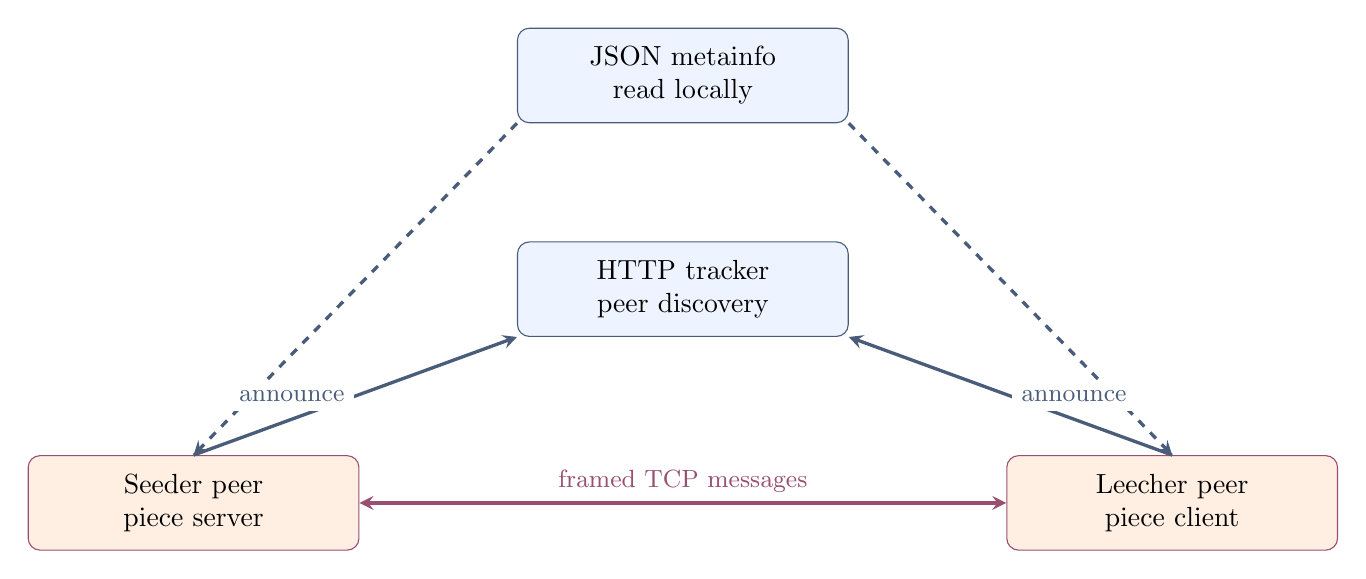
\begin{tikzpicture}[
    >=stealth,
    node distance=15mm and 20mm,
    component/.style={draw=Navy,fill=PaletteBlue!18!white,rounded corners=1.5mm,minimum width=42mm,minimum height=12mm,align=center},
    peer/.style={draw=Teal,fill=PalettePeach,rounded corners=1.5mm,minimum width=42mm,minimum height=12mm,align=center},
    flow/.style={very thick,->,Navy},
    direct/.style={very thick,<->,Teal}
  ]
    \node[component] (meta) {JSON metainfo\\read locally};
    \node[component,below=of meta] (tracker) {HTTP tracker\\peer discovery};
    \node[peer,below left=of tracker] (seed) {Seeder peer\\piece server};
    \node[peer,below right=of tracker] (leech) {Leecher peer\\piece client};

    \draw[flow,dashed] (meta.south west) -- (seed.north);
    \draw[flow,dashed] (meta.south east) -- (leech.north);
    \draw[flow] (seed.north) -- node[left,fill=white,font=\small] {announce} (tracker.south west);
    \draw[flow] (leech.north) -- node[right,fill=white,font=\small] {announce} (tracker.south east);
    \draw[direct] (seed.east) -- node[above,fill=white,font=\small] {framed TCP messages} (leech.west);
  \end{tikzpicture}%
  }
  \caption{Control-plane discovery through the tracker and direct peer-to-peer data transfer.}
  \label{fig:architecture}
\end{figure}

\subsection{Torrent lifecycle}

For each metainfo file, a worker performs the following sequence:

\begin{enumerate}
  \item load and validate the metainfo;
  \item scan local storage to establish the initial bitfield;
  \item start a peer server on a dedicated port;
  \item announce the \texttt{started} event to the tracker;
  \item discover peers and probe them with PING/PONG;
  \item request availability, express interest, and download missing pieces;
  \item verify every piece before storing it;
  \item send periodic progress announcements; and
  \item send \texttt{completed} and \texttt{stopped} events when applicable.
\end{enumerate}

Multiple metainfo files are represented as separate jobs in a thread pool. Their storage managers, network listeners, and transfer statistics remain distinct while they share the same application process.

\section{Metainfo and Tracker Design}
\label{sec:metainfo-tracker}

\subsection{Human-readable metainfo}

The project stores metainfo in JSON rather than the binary \texttt{.torrent} format. The \texttt{announce} field contains either one tracker URL or a list whose first entry is selected. The \texttt{info} dictionary contains the payload name, piece length, piece hashes, and either one total length or a list of files.

For total payload length $L_{\mathrm{total}}$ and piece length $L_{\mathrm{piece}}$, the expected number of pieces is

\begin{equation}
  N_{\mathrm{pieces}} =
  \left\lceil \frac{L_{\mathrm{total}}}{L_{\mathrm{piece}}} \right\rceil .
  \label{eq:piece-count}
\end{equation}

In multi-file mode, the listed files form one virtual byte stream. A piece may therefore begin near the end of one file and continue in the next. The parser validates required fields, positive lengths, hash syntax, piece count, and path components. Absolute paths, parent-directory traversal, and unsafe separators are rejected.

\subsection{Deterministic information hash}

The \texttt{info} dictionary is Bencoded with sorted dictionary keys and hashed with SHA-1:

\begin{equation}
  \mathrm{info\_hash} =
  \mathrm{SHA1}\!\left(\mathrm{Bencode}(\mathrm{info})\right).
  \label{eq:info-hash}
\end{equation}

This keeps torrent identity independent of the outer JSON layout while preserving deterministic encoding for the implemented field types.

\subsection{Tracker state and HTTP interface}

The tracker uses Python's \texttt{ThreadingHTTPServer}. Announce requests provide the information hash, peer identifier, listening port, uploaded and downloaded counters, remaining bytes, and an optional event. Binary identifiers are decoded from percent-encoded URL bytes.

Tracker state is grouped first by \texttt{info\_hash} and then by \texttt{peer\_id}. An \texttt{RLock} protects concurrent updates, while a cleanup thread removes peers that have not announced within the configured timeout. Successful responses contain the announce interval, complete and incomplete counts, and the peer list in Bencoded form.

\begin{importantnote}
The tracker is a discovery and state-coordination service. The implementation does not read, cache, or relay the shared payload.
\end{importantnote}

\section{Peer Protocol and Direct Transfer}
\label{sec:peer-protocol}

\subsection{Message framing}

TCP presents a byte stream rather than message boundaries. The implementation prefixes each JSON body with a four-byte unsigned length in network byte order:

\begin{equation}
  \mathrm{frame} =
  \mathrm{uint32\_be}(\lvert\mathrm{payload}\rvert)
  \mathbin{\Vert} \mathrm{JSON\ payload}.
  \label{eq:frame}
\end{equation}

The receive routine repeatedly reads until the declared number of bytes has arrived, so a message split across multiple TCP packets is reconstructed before JSON decoding. The default maximum frame size is eight MiB. The peer vocabulary includes \texttt{PING}, \texttt{PONG}, \texttt{BITFIELD}, \texttt{INTERESTED}, \texttt{UNCHOKE}, \texttt{REQUEST}, \texttt{PIECE}, and \texttt{ERROR}.

\subsection{Reachability and availability}

PING messages contain a random nonce and sender identifier. A valid PONG returns the same nonce, which lets the initiating peer associate the response with its probe. Once a peer is reachable, the client requests its bitfield, expresses interest when useful pieces are available, and waits for an unchoke response before requesting a piece.

\subsection{Piece exchange}

Piece bytes are Base64-encoded in the JSON body. This is easy to inspect but adds encoding overhead compared with a binary peer protocol. \Cref{alg:piece-cycle} summarizes the implemented validation cycle.

\begin{algorithm}[H]
  \caption{Validated piece request cycle}
  \label{alg:piece-cycle}
  \begin{algorithmic}[1]
    \Require peer endpoint, local piece manager, missing piece index $i$
    \State connect to the peer and request its bitfield
    \If{piece $i$ is unavailable}
      \State close the connection and select another peer
    \EndIf
    \State send \texttt{INTERESTED} and require \texttt{UNCHOKE}
    \State send \texttt{REQUEST} for piece $i$
    \State decode the returned Base64 piece bytes
    \State verify the declared index, length, and expected SHA-1 hash
    \If{verification succeeds}
      \State store the piece and update session counters
    \Else
      \State reject the bytes and log \texttt{HASH\_INVALID}
    \EndIf
  \end{algorithmic}
\end{algorithm}

\section{Piece Management, Concurrency, and Logging}
\label{sec:piece-management}

\subsection{Virtual file layout}

The piece manager converts the metainfo layout into a sequence of file segments with absolute offsets in the virtual torrent stream. Reads and writes are intersected with these segments, allowing one piece operation to span several local files. On startup, the manager scans existing storage and marks a piece available only when both its length and SHA-1 value match the metainfo.

For received bytes $p_i$ and expected hash $h_i$, acceptance requires

\begin{equation}
  \mathrm{SHA1}(p_i) = h_i.
  \label{eq:piece-integrity}
\end{equation}

A mismatch raises a dedicated error and leaves the piece unavailable. This check supports integrity within the project workflow; it does not authenticate the source peer.

\subsection{Concurrent services}

The tracker handles HTTP requests on separate threads and synchronizes shared swarm state. Each peer server accepts TCP connections and dispatches client handling concurrently. At application level, the torrent thread pool creates one worker per metainfo job, assigns a listening port, and tracks progress independently. A stop event coordinates graceful shutdown.

The design separates two measurements:

\begin{itemize}
  \item the piece manager represents durable availability inferred from local files; and
  \item transfer statistics represent bytes uploaded and downloaded during the current worker session.
\end{itemize}

This distinction prevents pre-existing valid pieces from being reported as bytes downloaded in the current run.

\subsection{Event logging}

The event logger records a file header followed by timestamped \texttt{event | time | description} rows. Inputs are normalized to one line, access is guarded by a per-path re-entrant lock, and updates are written to a temporary file before atomic replacement. Tracker and peer components use event names such as \texttt{ANNOUNCE\_RECEIVED}, \texttt{PING\_SENT}, \texttt{PIECE\_RECEIVED}, \texttt{HASH\_VALID}, and \texttt{PIECE\_STORED}.

\section{Validation Methodology}
\label{sec:validation}

The repository provides a standard-library-only test runner, \texttt{run\_all\_tests.py}. Tests create deterministic local payloads, bind tracker and peer services to loopback addresses, and write disposable outputs under ignored directories. No external tracker, dataset, or API is required.

\begin{table}[tbp]
  \centering
  \caption{Test groups executed by the supplied runner.}
  \label{tab:test-groups}
  \begin{tabularx}{\textwidth}{@{}p{0.28\textwidth}Y@{}}
    \toprule
    \tablehead{Test group} & \tablehead{Primary coverage} \\
    \midrule
    Metainfo & Single-file and multi-file creation, field validation, path safety, piece hashes, and cross-file boundaries. \\
    Logger & Header validation, concurrent writers, field sanitization, and atomic updates. \\
    Tracker state & Registration, completion, stopping, peer counts, timeout cleanup, and concurrent updates. \\
    Tracker HTTP & Announce parsing, binary URL values, response encoding, errors, and concurrent requests. \\
    Tracker client & URL generation, Bencode parsing, peer filtering, and progress events. \\
    Peer PING & Framing, partial reads, message-size limits, PING/PONG, and reachability results. \\
    Piece transfer & Bitfields, piece requests, valid storage, corrupt-piece rejection, and multi-file reconstruction. \\
    Torrent thread pool & Independent workers, concurrent downloads, progress accounting, and shutdown. \\
    Final integration & Demo preparation, two-torrent transfer, byte comparison, repository audit, and submission-archive checks. \\
    \bottomrule
  \end{tabularx}
\end{table}

The validation evidence is functional rather than performance-oriented. The materials do not specify throughput benchmarks, wide-area latency experiments, stress-test scale, or comparative baselines. Accordingly, no performance or scalability claim is made.

\section{Results and Observations}
\label{sec:results}

The supplied report records PASS outcomes for metainfo, tracker, peer, piece-transfer, multi-torrent, and integration checks. The integrated scenario used two torrents: a 4,099-byte single-file payload and a 3,164-byte multi-file bundle. The total transferred payload was therefore

\begin{equation}
  4{,}099 + 3{,}164 = 7{,}263\ \text{bytes}.
  \label{eq:total-payload}
\end{equation}

The integration assertions require both leecher workers to finish, both seeder workers to remain complete, session upload and download totals to equal 7,263 bytes, and three output files to match their sources. These checks validate the demonstrated workflow but should not be interpreted as a throughput benchmark.

\begin{reportfigure}[0.98\linewidth]{figures/tracker-http-traffic.png}
{Loopback capture of HTTP announce connections between peers and the tracker. File payloads are not present on this tracker connection.}
{fig:tracker-http}
\end{reportfigure}

\begin{reportfigure}[0.98\linewidth]{figures/peer-tcp-traffic.png}
{Loopback capture of direct TCP connections on the configured peer ports.}
{fig:peer-tcp}
\end{reportfigure}

\begin{figure}[tbp]
  \centering
  \begin{subfigure}[t]{0.49\textwidth}
    \centering
    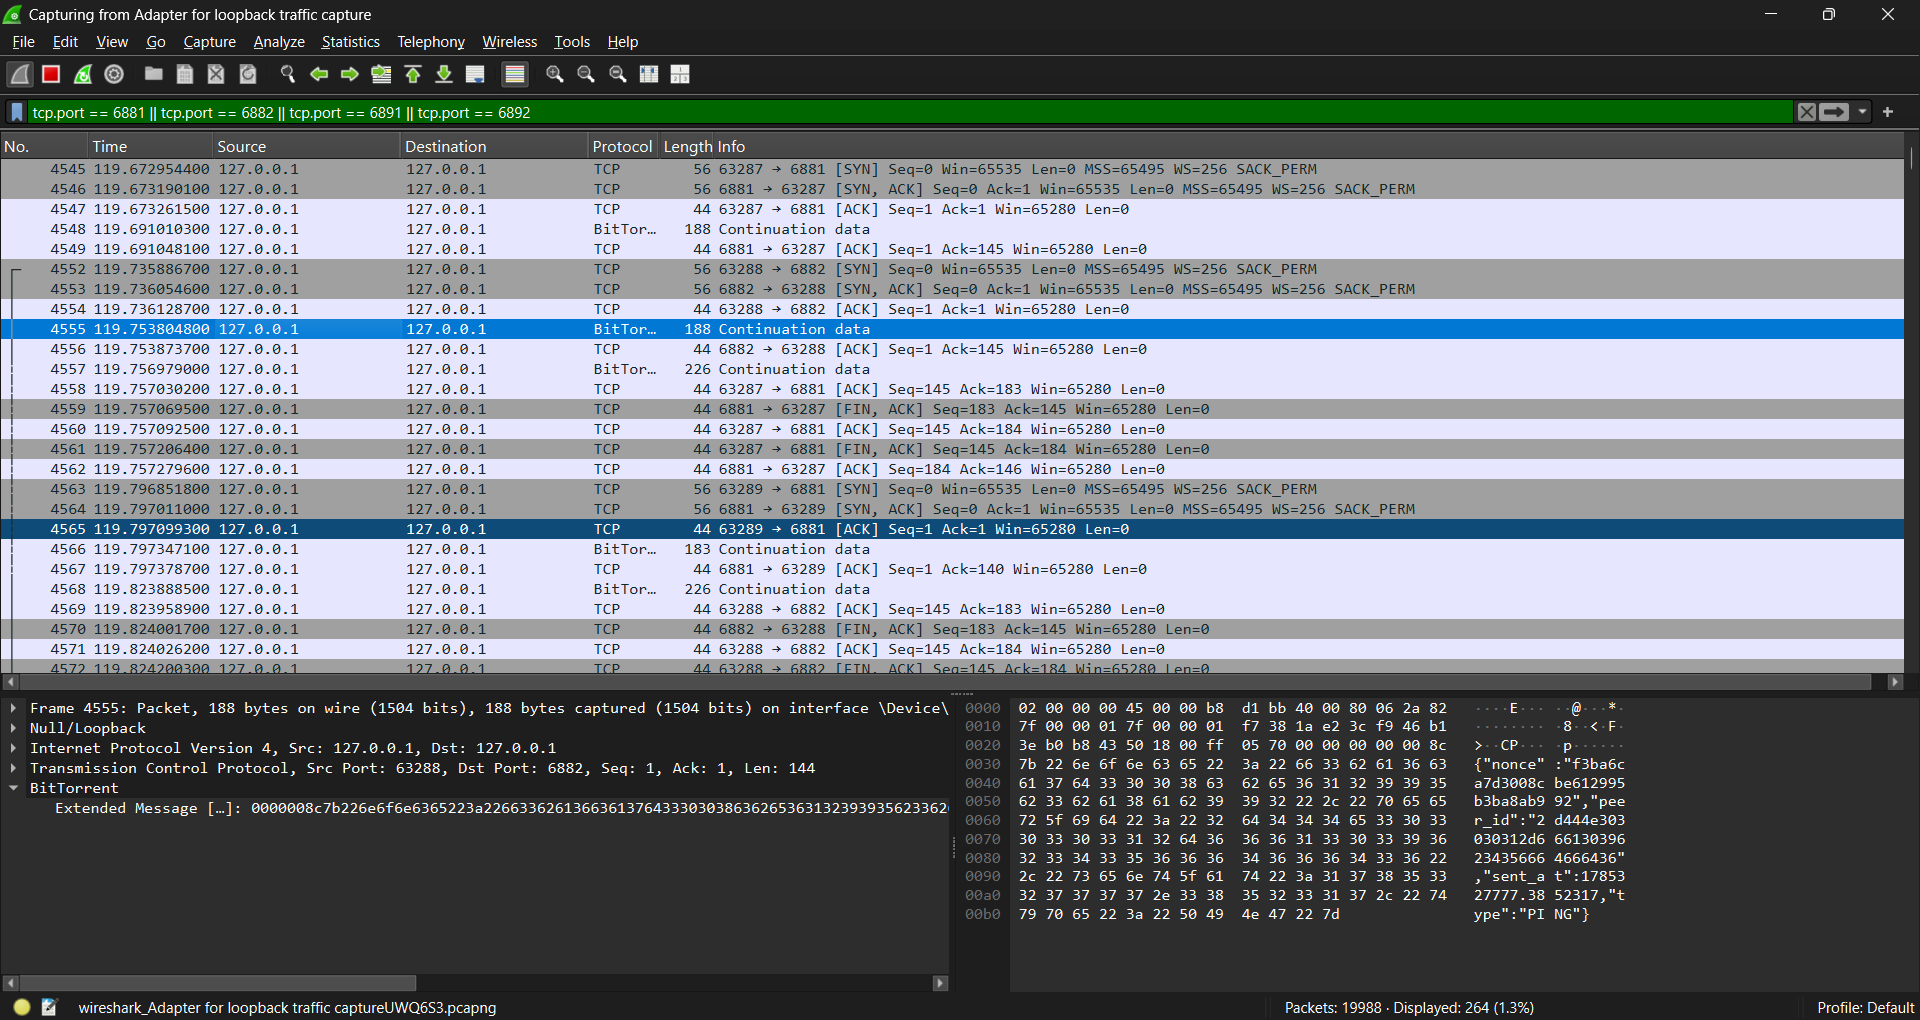
\includegraphics[width=\linewidth]{figures/ping-packet.png}
    \caption{Framed PING message in one peer connection.}
    \label{fig:ping-packet}
  \end{subfigure}\hfill
  \begin{subfigure}[t]{0.49\textwidth}
    \centering
    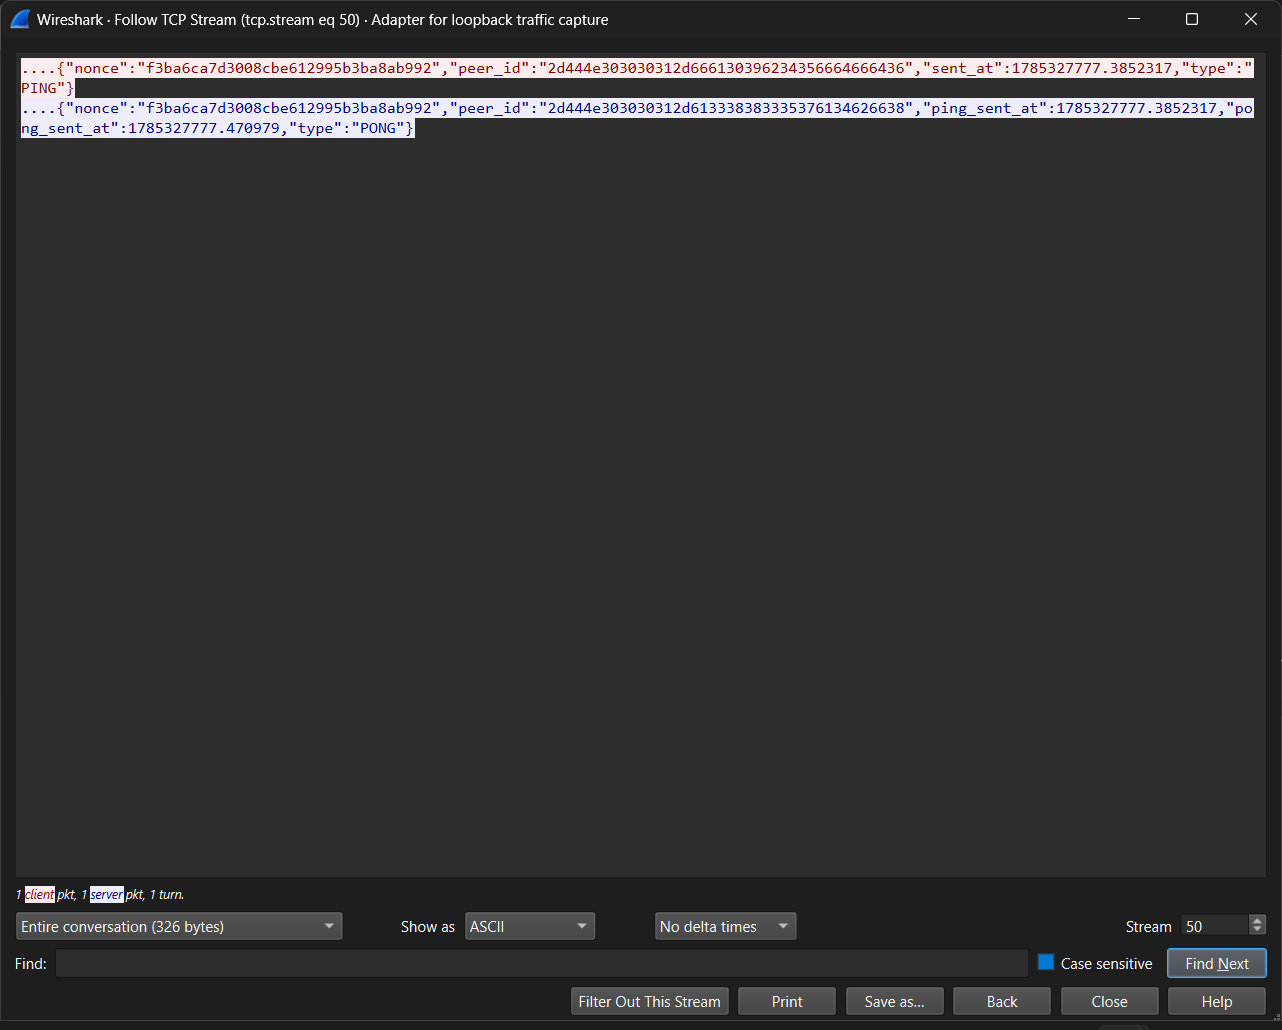
\includegraphics[width=\linewidth]{figures/ping-pong-stream.png}
    \caption{PING and PONG payloads in a followed TCP stream.}
    \label{fig:ping-stream}
  \end{subfigure}
  \caption{Packet-capture evidence for the custom peer reachability exchange.}
  \label{fig:ping-evidence}
\end{figure}

\Cref{fig:tracker-http,fig:peer-tcp} visually separates tracker traffic on port 8000 from direct traffic on peer ports. \Cref{fig:ping-evidence} shows the four-byte frame prefix followed by JSON application data and matching nonce values across PING/PONG. Packet segmentation itself is not used as a correctness criterion; application-level length, piece index, and hash checks provide the relevant validation.

\section{Limitations and Reproducibility}
\label{sec:limitations}

\subsection{Protocol limitations}

The implementation adopts selected BitTorrent concepts but defines its own metainfo and peer wire formats. JSON metainfo is not a standard binary \texttt{.torrent} file, and peer messages are length-prefixed JSON with Base64 piece data. The project does not implement rarest-first selection, end-game mode, tit-for-tat, NAT traversal, transport encryption, authentication, or a distributed hash table. Tracker and peer demonstrations use loopback networking.

SHA-1 verifies that a piece matches the metainfo, but the implementation does not establish who produced the metainfo or authenticate a remote peer. The supplied materials do not document an adversarial threat model, Internet deployment, sustained-load testing, or resource-isolation policy. These omissions limit any security or scalability interpretation.

\subsection{Reproduction procedure}

The implementation has no third-party Python dependency. A reproduction run requires Python 3.10 or newer and permission to bind local loopback ports. From the repository root, the complete test sequence is launched with:

\begin{lstlisting}[language=bash,numbers=none]
python run_all_tests.py
\end{lstlisting}

The tests create their own small payloads and output trees. Generated data, logs, caches, and submission archives are ignored by version control. The supplied materials do not specify the original Python patch version or a complete operating-system configuration, so exact-environment equivalence cannot be claimed.

\subsection{Publication boundaries}

The release excludes generated outputs, the redundant nested submission archive, bytecode caches, bundled fonts with unclear redistribution terms, the old PDF export, and six screenshots that display an absolute local path. Four project-generated loopback packet-capture screenshots are retained because they support the network-flow discussion without exposing the student identifier, email, credential, or private filesystem location.

\section{Conclusion}
\label{sec:conclusion}

The project provides a coherent educational implementation of tracker-assisted peer-to-peer file sharing. It separates peer discovery from payload transport, supports single-file and multi-file metainfo, frames peer messages over TCP, verifies each piece before storage, and coordinates several torrent workers concurrently. The test suite covers individual parsing and state components as well as complete loopback transfer and byte-for-byte reconstruction.

The implementation's strongest contribution is the integration of these concerns in a standard-library-only codebase with explicit event logging and reproducible local tests. Its scope is deliberately narrower than BitTorrent: custom JSON formats, loopback validation, and omitted production policies make it suitable as a networking course project rather than a general-purpose client.


\bibliography{references}

\clearpage
\appendix
\section{Execution Guide}
\label{app:execution}

\subsection{Automated validation}

Run all nine test groups from the repository root:

\begin{lstlisting}[language=bash,numbers=none]
python run_all_tests.py
\end{lstlisting}

The runner creates \texttt{test\_data/} and \texttt{test\_output/}; both are generated and ignored by Git.

\subsection{Automated integrated demo}

The integrated demo starts a loopback tracker, prepares deterministic single-file and multi-file payloads, launches seeder and leecher workers, and verifies the reconstructed files:

\begin{lstlisting}[language=bash,numbers=none]
python -m tools.end_to_end_demo \
  --workspace demo_workspace_integrated \
  --reset
\end{lstlisting}

\subsection{Manual Windows workflow}

The \texttt{demo/} directory contains five command files. Run them in numeric order. The tracker, seeder, and leecher commands are intentionally separated so their logs and progress can be observed in different terminals.

\begin{lstlisting}[language=bash,numbers=none]
01_prepare_demo.cmd
02_run_tracker.cmd
03_run_seed_peer.cmd
04_run_leecher_peer.cmd
05_verify_demo.cmd
\end{lstlisting}

All default endpoints use \texttt{127.0.0.1}. The tracker defaults to port 8000; the manual seeder and leecher commands begin their peer-port ranges at 6881 and 6891, respectively.


\end{document}
